\usetikzlibrary{calc}
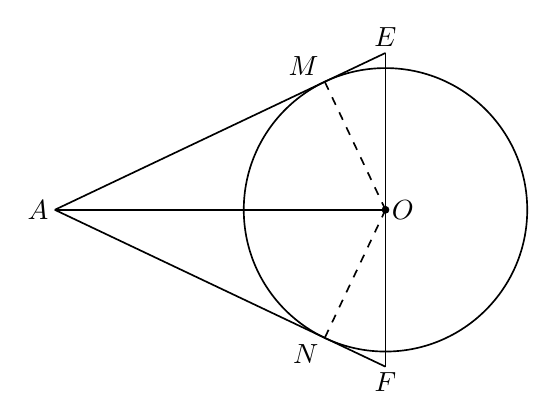
\begin{tikzpicture}[x=1cm,y=1cm,line width=.6pt,font=\normalsize]
\coordinate (O) at (0,0);
\coordinate (A) at (-4.2,0);
\coordinate (M) at (-0.7714,1.6263);
\coordinate (N) at (-0.7714,-1.6263);
\coordinate (E) at (0,1.9922);
\coordinate (F) at (0,-1.9922);
\draw[draw=black] (O) circle[radius=1.8cm];
\draw[draw=black] (A)--(E);
\draw[draw=black] (A)--(F);
\draw[draw=black] (A)--(O);
\draw[draw=black] (E)--(F);
\draw[draw=black,dashed] (O)--(M);
\draw[draw=black,dashed] (O)--(N);
\node[left=2pt,inner sep=0pt] at (A) {$A$};
\node[right=2pt,inner sep=0pt] at (O) {$O$};
\node[above=2pt,inner sep=0pt] at (E) {$E$};
\node[below=2pt,inner sep=0pt] at (F) {$F$};
\node[above left=2pt,inner sep=0pt] at (M) {$M$};
\node[below left=2pt,inner sep=0pt] at (N) {$N$};

% Explicit named circle-center points, painted after all region fills.
\fill (O) circle[radius=1.4pt];
\end{tikzpicture}
